\documentclass{article}
\title{Blanchard Ch.19}
\author{Dawei Wang}
\date{\today}
\usepackage{ctex}
\usepackage{amsmath}
\usepackage{amssymb}
\usepackage{graphicx} %插入图片的宏包
\usepackage{float} %设置图片浮动位置的宏包
\usepackage{subfigure} %插入多图时用子图显示的宏包
\begin{document}
	\maketitle

\section{产品市场的均衡}

\[
Y=C(Y-T)+I(Y,r)+G-IM(Y,\epsilon)/\epsilon+X(Y^*,\epsilon)
\]

产品市场均衡(IS):产出=对国内产品的需求。

定义“净出口”为:

\[
NX(Y,Y^*,\epsilon)=X(Y^*,\epsilon)-IM(Y,\epsilon)/\epsilon
\]

我们遵从关于进口和出口的假设,即净出口取决于国内产出$ Y $、外国产出$ Y^* $和实际汇率$\epsilon$:国内产出增加,进口增加净出口减少,外国产出增加将增加出口从而增加净出口,实际汇率的增加导致净出口的减少。(假设马歇尔-勒纳条件始终成立)。

利用净出口的定义,我们可以将这个均衡条件改写成:

\[
Y=C(Y-T)+I(Y,r)+G+NX(Y,Y^*,\epsilon)
\]

实际利率和实际汇率都影响需求,进而影响均衡产出。

实际利率的增加将导致投资支出的下降,从而对国内产品的需求下降。并通过乘数作用导致产出下降。

实际汇率的提高导致需求转向外国产品,从而导致净出口下降。净出口下降降低了对国内产品的需求,并通过乘数效应导致产出的下降。

\hspace*{\fill}

根据定义:$\epsilon=EP/P^*$。在短期假定国内外水平价格是固定的,因此名义汇率和实际汇率同步变动。

令$ P/P^*=1 $,从而$ \epsilon=E $。

由于假定国内价格水平是给定的,因此就不存在实际通货膨胀和预期通货膨胀。所以名义利率就等于实际利率:

\[
Y=C(Y-T)+I(Y,i)+G+NX(Y,Y^*,E)
\]

因此产品市场均衡表明产出与名义利率和名义汇率负相关。

\section{金融市场均衡}

考察金融市场开放的经济,必须将人们可以在国内债券和国外债券之间选择的事实一并考虑进来。

\subsection{国内债券和国外债券}

假设无论是国内还是国外的金融投资者都追求最高的预期回报率,无视风险差异。这就意味着,在均衡状态下国内债券和国外债券必须有同样的预期回报率,否则投资者就会只愿意购买一种债券而不是两种都有人买。这样就不能达到均衡。

这意味着下列套利条件一定会成立:

\[
(1+i_t)=(1+i^*_t)(\frac{E_t}{E^e_{t+1}})
\]

$ E_t $的出现源自这样一个事实:

为了购买外国债券,必须先将本币兑换成外币。

$ E^e_{t+1} $的出现源自于另一个事实:

为了在下一期收回资金,将不得不将外币换回本币。

\[
E_t=\frac{1+i_t}{1+i_t^*}E^e_{t+1}
\]

假定远期汇率是给定的,并将其标注为$ \overline{E}^e $。

\[
E=\frac{1+i}{1+i^*}\overline{E}^e
\]

这个关系式告诉我们现行汇率取决于国内利率、国外利率和预期的远期汇率:

国内利率的升高导致汇率升高;

国外利率升高导致汇率下降;

预期远期汇率的升高将导致现行汇率升高。

\begin{figure}[H] %H为当前位置,!htb为忽略美学标准,htbp为浮动图形
	\centering %图片居中
	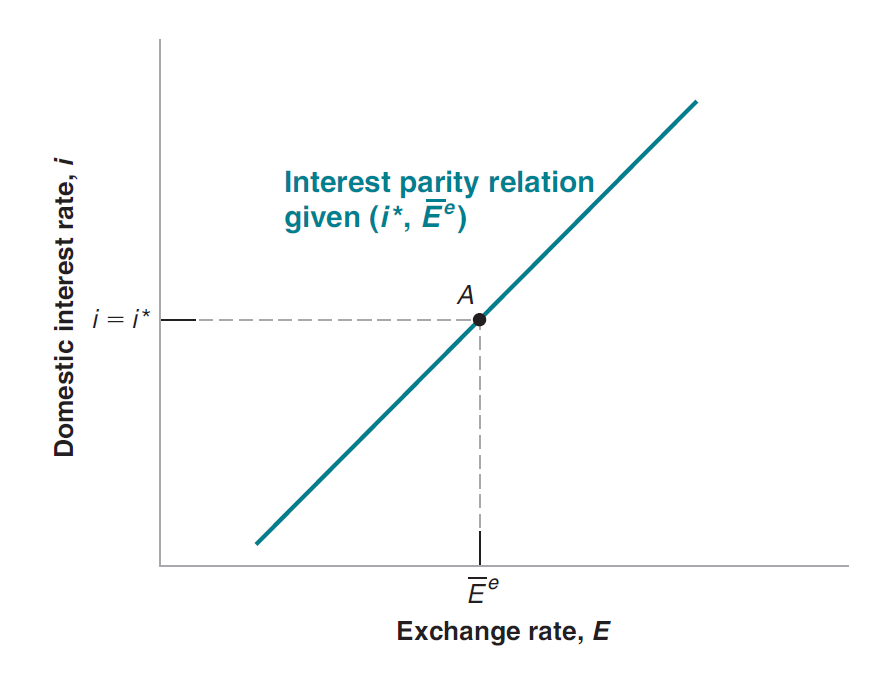
\includegraphics[width=1\textwidth]{19_1} %插入图片,[]中设置图片大小,{}中是图片文件名
	\caption{The Relation between
		the Interest Rate and the
		Exchange Rate Implied by
		Interest Parity} %最终文档中希望显示的图片标题
	\label{Fig.main2} %用于文内引用的标签
\end{figure}

\section{产品市场和金融市场的结合}

产品市场均衡:

\[
Y=C(Y-T)+I(Y,i)+G+NX(Y,Y^*,E)
\]

将利率i看作由中央银行规定的政策利率:

\[
i=\overline{i}
\]

并且,利率平价条件意味着国内利率和汇率之间存在正相关关系:

\[
E=\frac{1+i}{1+i^*}\overline{E}^e
\]

因此:IS和LM关系在开放经济中的版本为:

\[
IS:Y=C(Y-T)+I(Y,i)+G+NX(Y,Y^*,\frac{1+i}{1+i^*}\overline{E}^e)
\]

\[
LM:i=\overline{i}
\]

利率提高对产出的影响:

1. 对投资的直接影响,利率提高导致投资下降,从而导致对国内产品的需求减少,进而产出下降;

2. 通过汇率的效应:国内利率的提高使汇率升高,本币升值。本币升值使本国产品相对于外国产品来说变得昂贵,这导致净出口减少,进而对国内产品的需求减少,产出下降。

利率的提高直接使需求下降,也间接通过本币升值的负面效应使需求减少。

\begin{figure}[H] %H为当前位置,!htb为忽略美学标准,htbp为浮动图形
	\centering %图片居中
	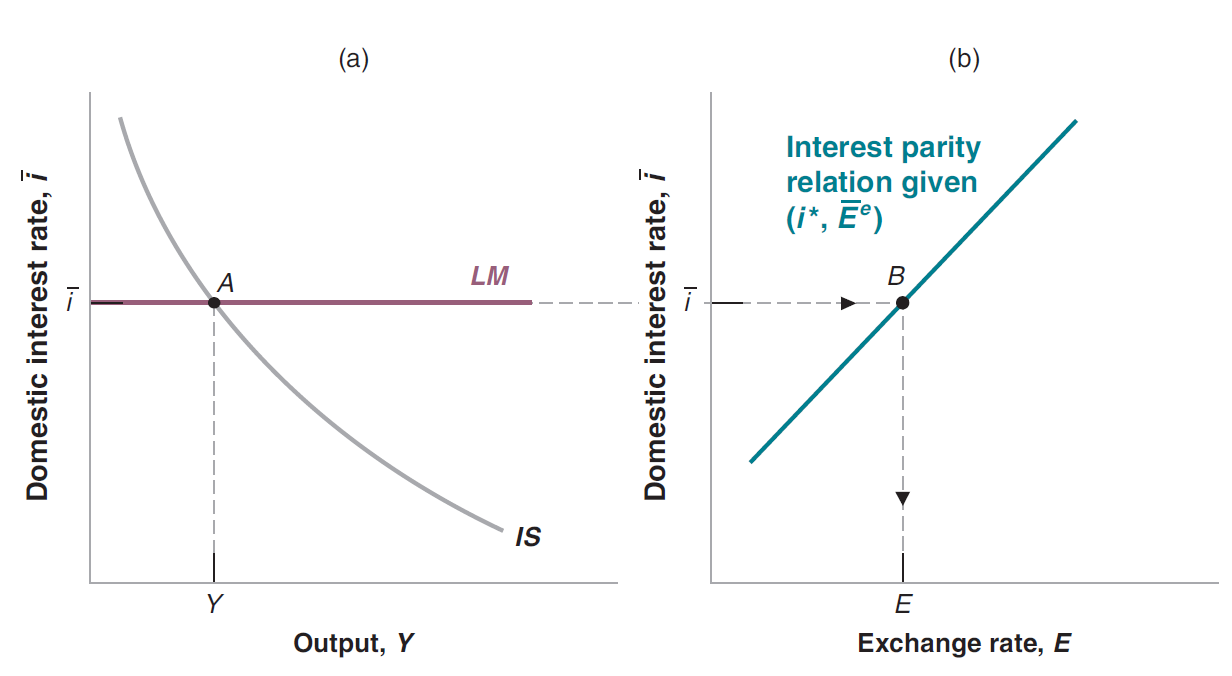
\includegraphics[width=1\textwidth]{19_2} %插入图片,[]中设置图片大小,{}中是图片文件名
	\caption{The IS-LM Model in
		an Open Economy} %最终文档中希望显示的图片标题
	\label{Fig.main3} %用于文内引用的标签
\end{figure}

开放经济中的LM关系和封闭经济中的完全一样。它是一条位于中央银行设定的利率水平处的水平线。

给定国外利率和预期远期汇率,则均衡利率决定了均衡汇率。

\section{开放经济中的政策效应}

\subsection{开放经济中的货币政策效应}

\begin{figure}[H] %H为当前位置,!htb为忽略美学标准,htbp为浮动图形
	\centering %图片居中
	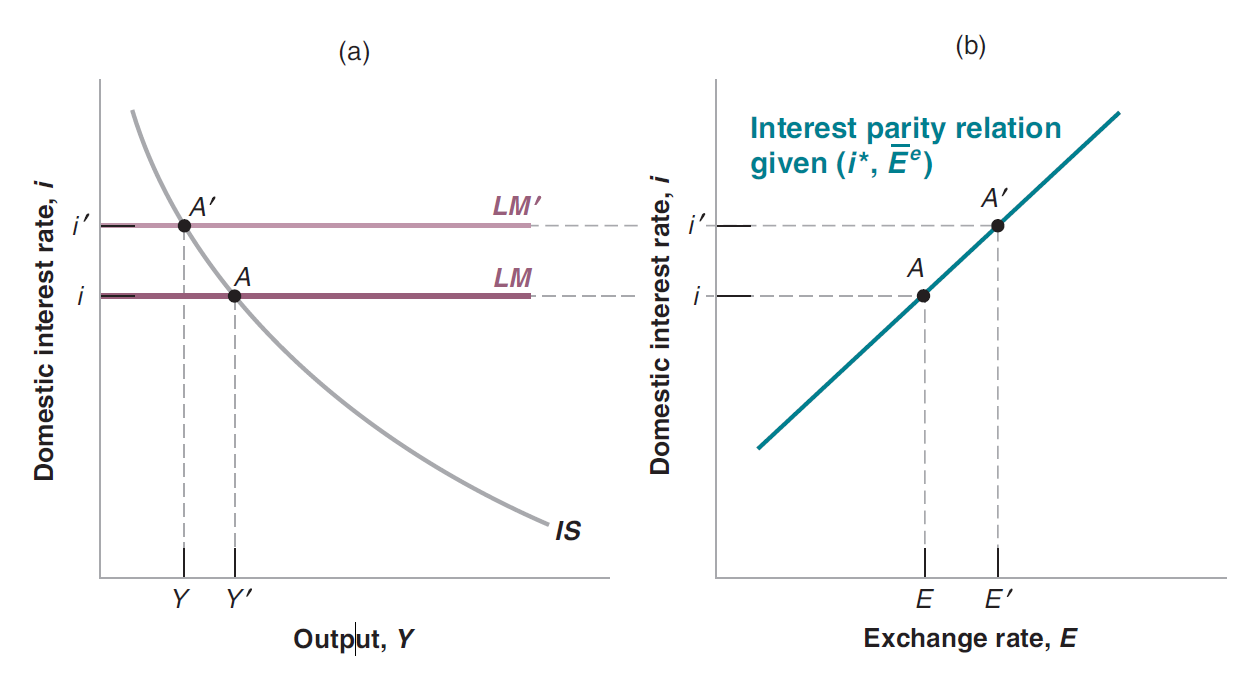
\includegraphics[width=1\textwidth]{19_3} %插入图片,[]中设置图片大小,{}中是图片文件名
	\caption{The Effects of an Increase
		in the Interest Rate} %最终文档中希望显示的图片标题
	\label{Fig.main4} %用于文内引用的标签
\end{figure}

如果中央银行决定提高国内利率,在给定的产出水平,利率提高,LM曲线上移到$ LM' $。IS曲线没有移动(只有)。均衡从A点移动到$ A' $。利率提高将导致本币升值。

在货币紧缩下,利率提高和本币升值都会导致需求和产出下降。

\subsection{开放经济中的财政效应}

\begin{figure}[H] %H为当前位置,!htb为忽略美学标准,htbp为浮动图形
	\centering %图片居中
	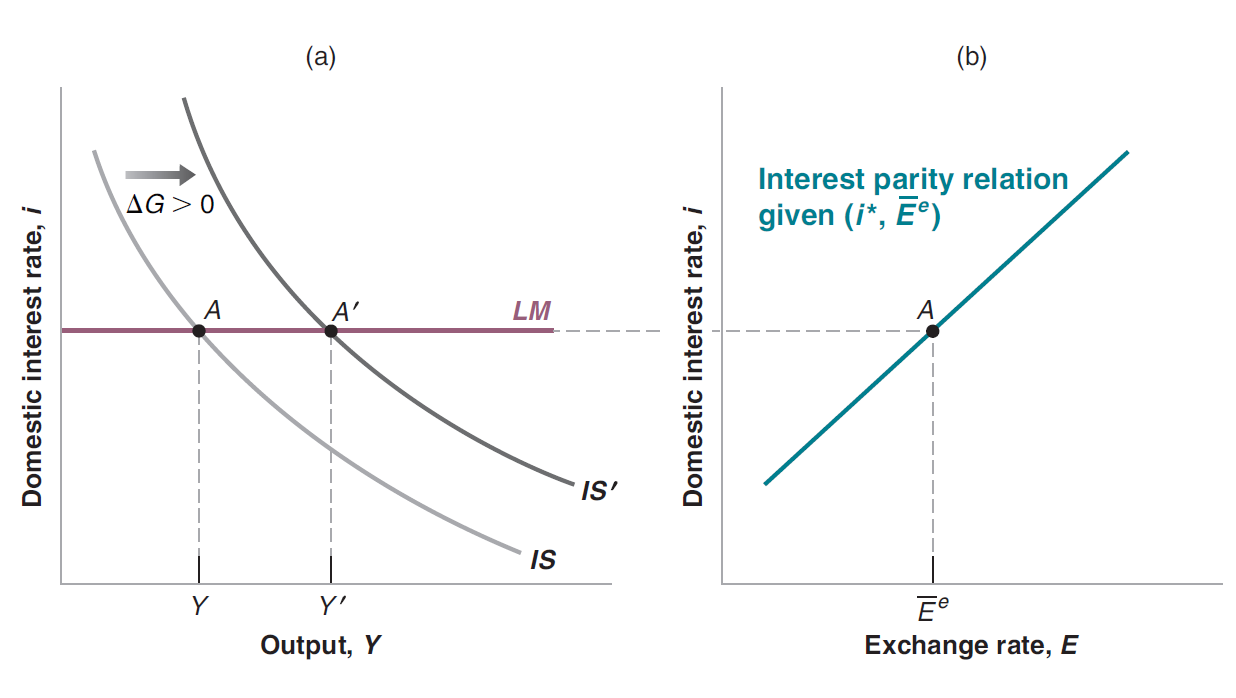
\includegraphics[width=1\textwidth]{19_4} %插入图片,[]中设置图片大小,{}中是图片文件名
	\caption{The Effects of an Increase
		in Government Spending
		with an Unchanged
		Interest Rate} %最终文档中希望显示的图片标题
	\label{Fig.main5} %用于文内引用的标签
\end{figure}

政府支出增加$ \Delta G>0 $,在每一个给定的利率下产出增加了,即IS曲线右移了,由于中央银行没有改变政策利率,因此LM曲线并没有移动。新的均衡点在$ A' $点,对应一个更高的产出水平和$ Y' $。因为利率不变,汇率也保持不变。所以当中央银行保持利率不变时,政府支出的增加会导致产出增加而汇率不变。

\hspace*{\fill}

需求的各组成部分变化:

消费和政府支出双双上升。消费的增加是因为收入增加,政府支出的增加是假设的;

投资上升,因为产出上升利率不变;

净出口下降:$ NX=NX(U,Y^*,E) $。外国产出不变,汇率不变。本国政府支出上升,导致本国产出上升,导致净出口下降。

\hspace*{\fill}

现在假设政府支G的增加发生在一个产出等于潜在产出$ Y_n $的经济体中。这种情况下政府担心政府支出G的增加可能会因为促使经济超过潜在产出水平而推高通货膨胀水平。为此,它会通过提高利率来做出应对。

\begin{figure}[H] %H为当前位置,!htb为忽略美学标准,htbp为浮动图形
	\centering %图片居中
	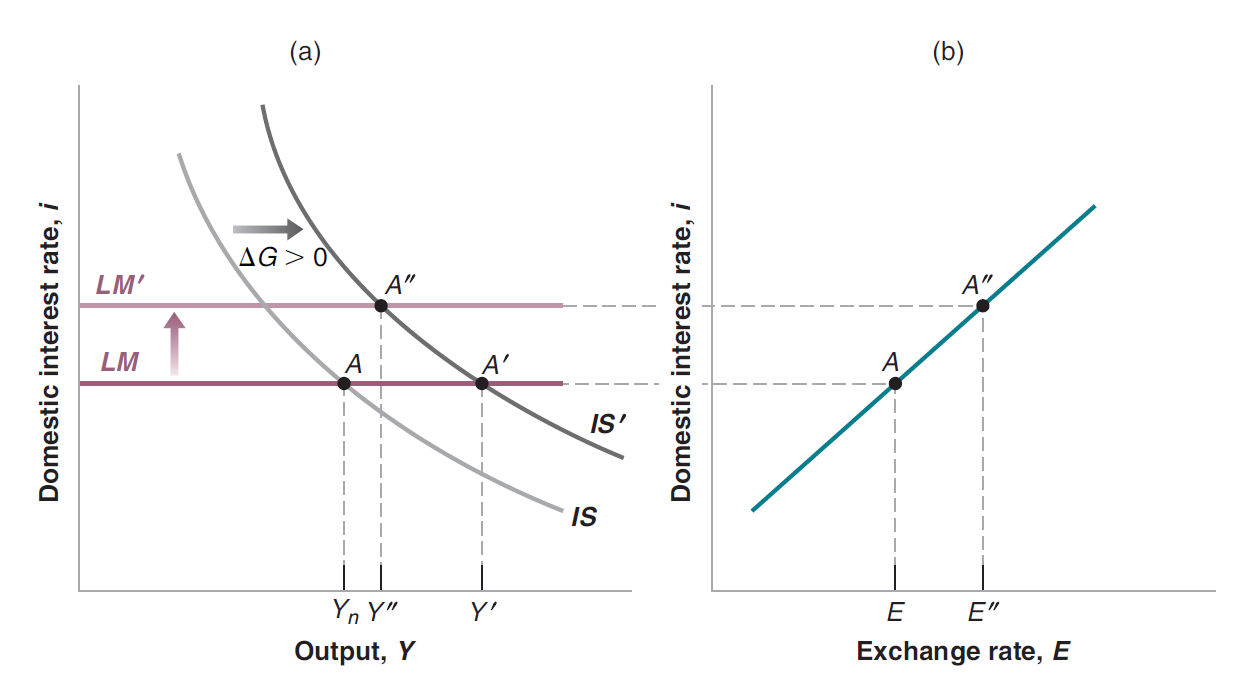
\includegraphics[width=1\textwidth]{19_5} %插入图片,[]中设置图片大小,{}中是图片文件名
	\caption{The Effects of an Increase
		in Government Spending
		when the Central Bank
		Responds by Raising the
		Interest Rate} %最终文档中希望显示的图片标题
	\label{Fig.main6} %用于文内引用的标签
\end{figure}

如果中央银行在增加政府支出的同时辅以利率的提高,产出的增加将会减少,从$ Y_n $增加到$ Y'' $,汇率将会从E提高到$ E'' $。

需求的各个部分的变化:

消费和政府支出双双上升,消费的增加是因为收入的增加,而政府指出的增加是我们假定的;

投资的变化现在不清楚。投资取决于产出和利率:$ I=I(Y,i) $。这里产出增加但利率也增加;

净出口下降:产出增加提高了进口,利率上升引起汇率升值提高了进口同时降低了出口。预算赤字导致贸易赤字(但是贸易赤字是否大于政策利率保持不变时的情况不清楚。汇率升值使情况恶化,但是利率提高导致产出增幅变小,因此进口的增幅也变小。)


\section{固定汇率制}

\subsection{钉住、爬行钉住、带状范围、欧洲货币体系和欧元}

在一个极端上,国家实行完全浮动的汇率制度,如美、英、日、加,这些国家没有明确的汇率目标。

另一个极端是实行固定汇率制度的国家。这些国家将汇率与一些外国货币保持固定的比率。有一些国家采用本币钉住(peg)美元。

“固定”并不是说实行固定汇率的国家的汇率从来不变动,而是变动很少。把固定汇率制度下汇率的下降叫作认为贬值或低估而不是市场贬值,把固定汇率制度下汇率的升高叫作人为高估或高估而不是市场升值。

在这两类极端的国家之间是对汇率目标做出不同程度承诺的国家。例如一些执行爬行钉住(crawling peg)汇率制度。这些国家的通胀率通常要超过美国的通胀率。如果它们将本国名义汇率钉住美元,那么因为它们的国内价格水平的增长要快于美国,因而会导致持续的实际升值,从而使它们的产品失去竞争力。为了避免这种影响,这些国家选择了一个事先确定的对美元的贬值率。它们选择相对于美元“爬行”(缓慢地移动)。

另外一种汇率安排是一些国家集团将彼此之间的双边汇率保持在一定范围内。最显著的例子是欧洲货币体系(European Monetary System,EMS),该体系决定了1978~1998年欧盟内部汇率的变动。在EMS规则下,成员国同意其对该体系内其他国家的汇率维持在一个很小的范围之内,即围绕一个给定的中间平价(central parity)的带状范围(bands)。中间平价的变动以及特定货币的贬值和升值也会发生,但是必须得到其他成员国的普遍同意。

\subsection{固定汇率制度下的货币政策}

不管钉住还是不钉住,汇率和名义利率都必须满足利率平价条件:

\[
(1+i_t)=(1+i^*)\frac{E_t}{E_{t+1}^e}
\]

现在假设一个国家把汇率钉在一个选定的值$ \overline{E} $,所以即期汇率为$ E_t=\overline{E} $。如果金融市场和外汇市场均相信汇率将保持在钉住值,那么预期远期汇率$ E^e_{t+1} $也等于$ \overline{E} $,利率平价条件变为:

\[
(1+i_t)=(1+i_t^*)\Rightarrow i_t=i^*_t
\]

在固定汇率制度下,中央银行将放弃货币政策这一政策工具。固定汇率制下国内利率必须等于国外利率。(这些结果在很大程度上依赖于利率平价条件,而这个条件相应地又依赖于完全资本流动假设,即金融投资者追求最高的预期回报率。)

\subsection{固定汇率制下地财政政策}

当中央银行钉住汇率时,政府支出增加地效应和完全浮动汇率制度下的情况一样。因为如果支出增加没有伴随利率变动,那么汇率就不会变动。所以当政府支出增加时,无论该国是否钉住汇率,结果都没有区别。固定汇率制度和完全浮动汇率制的区别在于中央银行的应对能力。

\hspace*{\fill}

通过把汇率固定下来,一个国家就放弃了一个纠正贸易不平衡或者改变经济活动水平的有力工具;

通过承诺一个特定的汇率,也使国家放弃了对利率的控制;

虽然国家保持了对财政政策的控制,但是单一的政策工具是远远不够的。











\end{document}